% !TeX root = ../main.tex
No cotidiano, o ser humano raramente raciocina por categorias absolutamente rígidas. Ao avaliar se um dia está quente, se uma pessoa é alta ou se uma imagem está nítida, por exemplo, normalmente não é pensado em termos de “pertence” ou “não pertence”, como estabelece a lógica clássica dos conjuntos. Em vez disso, é pensado em graus: algo pode ser um pouco quente, muito quente, relativamente alto ou razoavelmente nítido. É justamente essa forma mais gradual e flexível de interpretar a realidade que motiva a teoria dos conjuntos fuzzy. Ao permitir que um elemento pertença a um conjunto com diferentes graus de pertinência, essa abordagem se torna mais adequada para representar incertezas, imprecisões e transições suaves entre categorias. Neste capítulo, são apresentados os principais conceitos da teoria dos conjuntos fuzzy e dos sistemas baseados em regras fuzzy, que são utilizadas no desenvolvimento deste trabalho.

A teoria dos conjuntos fuzzy, introduzida por Lotfi A. Zadeh em 1965 \cite{zadeh1965fuzzy}, é uma extensão da teoria clássica dos conjuntos, permitindo a representação de incerteza e imprecisão. Diferentemente dos conjuntos clássicos, em que um elemento pertence ou não a um conjunto, nos conjuntos fuzzy cada elemento possui um grau de pertinência, variando entre 0 e 1. Essa abordagem é especialmente útil em análise de imagens, em que as características dos objetos podem ser ambíguas ou imprecisas, dependendo do contexto, e a classificação binária pode não ser suficiente para capturar a complexidade dos dados. As definições e propriedades dos conjuntos fuzzy presentes neste capítulo foram baseadas em \citeonline{fuzzy}.

\section{Conjuntos Fuzzy}
Um \textit{subconjunto fuzzy} $A$ de um conjunto universo $X$ é definido por uma função de pertinência $\mu_A$ que atribui a cada elemento $x \in X$ um valor $\mu_A(x) \in [0, 1]$, representando o grau de pertencimento de $x$ ao conjunto $A$. Assim:
$$
\mu_A: X \rightarrow [0, 1].
$$
O valor $\mu_A(x) = 0$ indica que $x$ não pertence ao conjunto $A$, enquanto $\mu_A(x) = 1$ indica que $x$ pertence completamente ao conjunto. Valores intermediários representam graus parciais de pertencimento, permitindo uma representação mais rica e flexível de conceitos vagos ou imprecisos.

\begin{exemplo}
    \label{ex:fuzzy}
Considere o conjunto universo $X$ representando a temperatura em graus Celsius, e o conjunto fuzzy $A$ representando a categoria ``temperatura alta". A função de pertinência $\mu_A$ pode ser definida da seguinte forma:
\begin{equation}
    \label{eq:pertinencia}
\mu_A(x) = \begin{cases}
0 & \text{se } 0^\circ \text{C} \leq x \leq 20^\circ \text{C} \\
\frac{x - 20}{10} & \text{se } 20^\circ \text{C} < x < 30^\circ \text{C} \\
1 & \text{se } x \geq 30^\circ \text{C}
\end{cases}.
\end{equation}
\end{exemplo}
Neste exemplo, temperaturas de $20^\circ$C ou menos não são consideradas altas ($\mu_A(x) = 0$), enquanto temperaturas de $30^\circ$C ou mais são consideradas completamente altas ($\mu_A(x) = 1$). Temperaturas entre $20^\circ$C e $30^\circ$C têm um grau de pertinência que varia linearmente entre 0 e~1, refletindo a natureza gradual do conceito de temperatura alta. Na Figura \ref{fig:pertinencia} é ilustrado o gráfico da função de pertinência $\mu_A(x)$.
\begin{figure}[htpb]
    \centering
    \caption{Função de pertinência $\mu_A(x)$ para o conjunto fuzzy ``temperatura alta".}
    \includegraphics*[width=0.6\textwidth]{graf_func_pertinencia.png}
    \label{fig:pertinencia}
\end{figure}
Pode-se observar que a função de pertinência $\mu_A(x)$ é uma função crescente para valores entre $20^\circ$C e $30^\circ$C, refletindo a ideia de que à medida que a temperatura aumenta, o grau de pertencimento ao conjunto fuzzy ``temperatura alta" também aumenta.

\subsection{Operações entre Conjuntos Fuzzy}
Os conceitos e definições que sucedem este capítulo são essenciais para a compreensão da U-Net Fuzzy, desenvolvida posteriormente. As operações entre conjuntos fuzzy, como união, interseção e complemento, são definidas de maneira a preservar a estrutura fuzzy. A união de dois conjuntos clássicos $A$ e $B$ é dada por:
$$A \cup B = \{x \in U;x \in A \ \text{ou} \ x \in B\},$$
enquanto a interseção é definida por:
$$A \cap B = \{x \in U;x \in A \ \text{e} \ x \in B\}.$$
O complemento de um conjunto clássico $A$ é dado por:
$$\bar{A} = \{x \in U; x \notin A\}.$$
Essas três operações têm respectivamente as funções características, $\forall x \in X$
$$
u_{A \cup B}(x) = \max(u_A(x), u_B(x)), \quad
u_{A \cap B}(x) = \min(u_A(x), u_B(x)), \quad
u_{\bar{A}}(x) = 1 - u_A(x). 
$$

A união, interseção e complemento de conjuntos fuzzy são definidas de maneira análoga, utilizando as funções de pertinência.

\begin{definicao}
    \label{def:operacoesfuzzy}
    Sejam $A$ e $B$ conjuntos fuzzy em um conjunto universo $X.$ A união, interseção e complemento de $A$ e $B$, denotadas por $A \cup B$, $A \cap B$ e $A'$, respectivamente, são as funções de pertinência, presentes na Figura \ref{fig-cap2:conjuntosfuzzy}, definidas por:
$$\mu_{A \cup B}(x) = \max(\mu_A(x), \mu_B(x)) \quad \text{para todo } x \in X,$$
$$\mu_{A \cap B}(x) = \min(\mu_A(x), \mu_B(x)) \quad \text{para todo } x \in X,$$
$$\mu_{\bar{A}}(x) = 1 - \mu_A(x) \quad \text{para todo } x \in X.$$
\end{definicao}

De fato, observa-se que a definição (\ref{def:operacoesfuzzy}) é uma extensão natural das operações clássicas de união, interseção e complemento para o contexto dos conjuntos fuzzy. Nos conjuntos clássicos, a função de pertinência assume apenas valores binários, ou seja:
$$
\mu_A(x) = \begin{cases}1, & \text{se } x \in A \\ 0, & \text{se } x \notin A \end{cases}.
$$
Assim, se $A= \{1,2,3\}$ e $B = \{3,4,5\}$, é obtida a seguinte tabela:
\begin{center}
\begin{tabular}{cccccc}
\hline
$x$ & $\mu_A(x)$ & $\mu_B(x)$ & $\mu_{A \cup B}(x)$ & $\mu_{A \cap B}(x)$ & $\mu_{\bar{A}}(x)$ \\
\hline
1 & 1 & 0 & 1 & 0 & 0 \\
\hline
2 & 1 & 0 & 1 & 0 & 0 \\
\hline
3 & 1 & 1 & 1 & 1 & 0 \\
\hline
4 & 0 & 1 & 1 & 0 & 1 \\
\hline
5 & 0 & 1 & 1 & 0 & 1 \\
\hline
\end{tabular}
\end{center}
Observa-se que os valores obtidos para $\mu_{A \cup B}(x)$, $\mu_{A \cap B}(x)$ e $\mu_{\bar{A}}(x)$ correspondem exatamente à definição (\ref{def:operacoesfuzzy}) de união, interseção e complemento, respectivamente.  Na Figura \ref{fig-cap2:conjuntosfuzzy} são ilustrados os gráficos das funções de pertinência para a união, interseção e complemento dos conjuntos fuzzy $A$ e $B$.
\begin{figure}[htpb]
    \centering
    \caption{Operações entre conjuntos fuzzy.}
    
\includegraphics[width=1\textwidth]{operacoes_fuzzy.png}
    \caption*{\footnotesize Fonte: Adaptado de \cite{fuzzy}.}
    \label{fig-cap2:conjuntosfuzzy}
\end{figure}
Os pontos presentes nos gráficos da Figura \ref{fig-cap2:conjuntosfuzzy}(a) e Figura \ref{fig-cap2:conjuntosfuzzy}(b) representam a região dos valores de $\mu_A(x)$ e $\mu_B(x)$ obtidos após as operações de união e interseção, respectivamente.

\subsection{Normas Triangulares}
As normas triangulares são generalizações dos operadores união e intersecção.

\begin{definicao}
Uma co-norma triangular (s-norma) é uma operação binária $S: [0, 1] \times [0, 1] \rightarrow [0, 1]$ que satisfaz as seguintes propriedades:
\begin{itemize}
    \item Comutatividade: $xSy = ySx$
    \item Associatividade: $xS(ySz) = (xSy)Sz$
    \item Monotonicidade: Se $x \leq x'$ e $y \leq y'$, então $xSy \leq x'Sy'$
    \item Condição de fronteira: $xS0 = x$ e $xS1 = 1$
\end{itemize}
\end{definicao}

\begin{exemplo}
    União Padrão: $S: [0,1] \times [0,1] \to [0,1]$ com $xSy = \max(x, y)$ é uma co-norma triangular. 
\end{exemplo}
    De fato, $max(x,y) = max(y,x)$, $max(x, max(y,z)) = max(max(x,y), z)$, $max(x,y) \leq max(x',y')$ se $x \leq x'$ e $y \leq y'$, $max(x,0) = x$ e $max(x,1) = 1$ para todo $x \in [0,1]$.

\begin{definicao}
Uma norma triangular (t-norma) é uma operação binária $T: [0, 1] \times [0, 1] \rightarrow [0, 1]$ que satisfaz as seguintes propriedades:
\begin{itemize}
    \item Comutatividade: $xTy = yTx$
    \item Associatividade: $xT(yTz) = (xTy)Tz$
    \item Monotonicidade: Se $x \leq x'$ e $y \leq y'$, então $xTy \leq x'Ty'$
    \item Condição de fronteira: $0Tx = 0$ e $1Tx = x$
\end{itemize}
\end{definicao}
\begin{exemplo}
    Intersecção Padrão: $T: [0,1] \times [0,1] \to [0,1]$ com $xTy = \min(x,y)$ é uma norma triangular.
\end{exemplo}
De fato, observa-se que $min(x,y) = min(y,x)$, $min(x, min(y,z)) = min(min(x,y), z)$, $min(x,y) \leq  min(x',y')$ se $x \leq x'$ e $y \leq y'$, $min(0,x) = 0$ e $min(1,x) = x$ para todo $x \in [0,1]$.


\subsection{Níveis de um Conjunto Fuzzy}
\begin{definicao}
    Sejam $A$ um conjunto fuzzy e $\alpha \in (0,1]$. O $\alpha$-nível de $A$, denotado por $[A]^{\alpha}$, é o conjunto clássico definido por:
$$[A]^{\alpha} = \{x \in X \mid \mu_A(x) \geq \alpha\}.$$
\end{definicao}

\begin{definicao}
    O suporte de um conjunto fuzzy $A$ são todos os elementos de $X$ que têm grau de pertinência maior que zero em $A$, ou seja:
$$supp(A) = \{x \in X \mid \mu_A(x) > 0\}.$$
\end{definicao}

\begin{definicao}
    O nível zero de um conjunto fuzzy $A$ do universo $X$, em que $X$ é um espaço topológico, é o fecho topológico do suporte de $A$, ou seja:
$$[A]^0 = \overline{supp(A)}.$$
\end{definicao}




\begin{exemplo}
Seja $A$ o conjunto fuzzy representando a categoria ``temperatura alta" do Exemplo \ref{ex:fuzzy}, dada pela função de pertinência (\ref{eq:pertinencia}).
\end{exemplo}
 O $\alpha$-nível de $A$ para $\alpha = 0,5$ é dado por:
$$[A]^{0,5} = \{x \in \mathbb{R} \mid \mu_A(x) \geq 0,5\}.$$

Neste caso, tem-se:
$$\mu_A(x) \geq 0,5 \implies \frac{x - 20}{10} \geq 0,5 \implies x \geq 25^\circ C.$$

Portanto, o $\alpha$-nível de $A$ para $\alpha = 0,5$ é o intervalo $[25^\circ C, \infty)$, representando a ``temperatura alta" com um grau de pertinência de pelo menos 0,5.

O suporte de $A$ é dado por:
$$\mu_A(x) > 0 \implies \frac{x - 20}{10} > 0 \implies x > 20^\circ C.$$

Portanto, o suporte de $A$ é o intervalo $(20^\circ C, \infty)$, representando a ``temperatura alta" que tem um grau de pertinência maior que zero em $A$.


\subsection{Números Fuzzy}
Um número fuzzy é um subconjunto fuzzy do conjunto dos números reais, caracterizado por uma função de pertinência que atribui a cada número real um grau de pertencimento. Os números fuzzy são frequentemente utilizados para representar quantidades imprecisas ou vagamente definidas.

\begin{definicao}
Um conjunto fuzzy $N$ é chamado de número fuzzy quando o conjunto universo, em que $N$ é definido, é o conjunto dos números reais $\mathbb{R}$, e a função de pertinência $\mu_N$ é tal que:
\begin{itemize}
    \item $\mu_N(x) = 1$ para pelo menos um valor $x$ de $supp(N)$;
    \item $[N]^{\alpha}$ é um intervalo fechado para todo $\alpha \in (0,1]$;
    \item O suporte de $N$ é limitado.
\end{itemize}
\end{definicao}

\begin{exemplo}
    Um número fuzzy $A$ é dito trapezoidal se o gráfico de sua função de pertinência tem a forma de um trapézio. A função de pertinência de um número fuzzy trapezoidal pode ser definida por quatro parâmetros $a, b, c, d$ (com $a \leq b \leq c \leq d$) da seguinte forma:
\end{exemplo}
$$\mu_A(x) = \begin{cases}
\frac{x - a}{b - a}, & \text{se } a < x < b \\
1, & \text{se } b \leq x < c \\
\frac{d - x}{d - c}, & \text{se } c \leq x < d \\
0, & \text{caso contrário} 
\end{cases}$$
Neste exemplo, o número fuzzy $A$ é representado por um trapézio definido pelos parâmetros $a, b, c, d$. Para $a < x < b$, a função de pertinência aumenta linearmente de 0 a 1, indicando um aumento gradual no grau de pertencimento. Para $b \leq x < c$, a função de pertinência é constante em 1, indicando que esses valores pertencem completamente ao conjunto fuzzy. Para $c \leq x < d$, a função de pertinência diminui linearmente de 1 a 0, indicando uma diminuição gradual no grau de pertencimento.

\begin{exemplo}
    Um número fuzzy $A$ é dito  gaussiano se  o gráfico de sua função de pertinência tem a forma de uma curva gaussiana, dada por:
    \end{exemplo}
    \textcolor{red}{mudar aqui}
    \begin{equation}
        \label{eq:gaussiana}
        \mu_A(x) = 
        \begin{cases}
        e^{-\frac{(x - c)^2}{2\sigma^2}}, \ \text{se} \ c-\sigma \le x \le c+ \sigma , \\
        0, \ \text{caso contrário}
        \end{cases},
    \end{equation}
    em que $c$ é o centro do número fuzzy e $\sigma$ é o desvio padrão, que controla a largura da curva. Na Figura \ref{fig:gaussiana} é ilustrado o gráfico da função de pertinência de um número fuzzy gaussiano.
    \begin{figure}[htpb]
        \centering
        \caption{Função de pertinência de um número fuzzy gaussiano.}
        
\includegraphics[width=0.6\textwidth]{cap2/gauss.png}
        \label{fig:gaussiana}
    \end{figure}
    O número fuzzy gaussiano é caracterizado por uma função de pertinência suave e contínua, que atinge seu valor máximo em $x = c$ e decresce à medida que $x$ se afasta de $c$. Observa-se que o gráfico da função é limitado para o intervalo $[c - \sigma, c + \sigma]$, para que seja satisfeita a condição de suporte limitado.






\section{Sistema Baseado em Regras Fuzzy}
\label{sec:sbrf}

Para que seja possível mesclar os conceitos de redes neurais com a teoria fuzzy, é necessário compreender a estrutura e o funcionamento de um Sistema Baseado em Regras Fuzzy - SBRF. Um SBRF é um sistema que utiliza a teoria dos conjuntos fuzzy para produzir saídas a partir de entradas dadas por conjuntos fuzzy \cite{fuzzy}. Tais sistemas foram desenvolvidos com o objetivo de imitar o comportamento humano considerando que o conhecimento e as ações humanas são apoiadas em uma sequência de regras linguísticas, traduzidas por um conjunto de regras. As regras formuladas pelo ser humano são usualmente da forma: 
\begin{center}
\textit{SE} (um conjunto de condições é satisfeito) \textit{ENTÃO} (um conjunto de consequências pode ser inferido).
\end{center}

Para que seja possível formalizar as regras fuzzy, é necessário definir o conceito de relação fuzzy.
\begin{definicao}
    Uma relação fuzzy $R$ é um subconjunto fuzzy do produto cartesiano entre conjuntos universos $X_1, \ X_2, \ \cdots \ X_n$, ou seja, $R \subseteq X_1 \times X_2 \times \cdots \times X_n$. O produto cartesiano fuzzy $A_1 \times A_2 \times \cdots \times A_n$ dos subconjuntos fuzzy $A_1, A_2, \cdots, A_n$ de $X_1, X_2, \cdots, X_n$, respectivamente, é a relação fuzzy $R$ cuja função de pertinência é dada por:
$$\mu_R(x_1, x_2, \cdots, x_n) = \min(\mu_{A_1}(x_1), \mu_{A_2}(x_2), \cdots, \mu_{A_n}(x_n)).$$
\end{definicao}

\subsection{Regras e Inferência Fuzzy}
Uma regra fuzzy é uma sentença da forma ``SE $X$ é $A$ ENTÃO $Y$ é $B$", em que $A$ e $B$ são conjuntos fuzzy em $X$ e $Y$, respectivamente. Tal regra pode ser interpretada como uma relação fuzzy $R$ entre os conjuntos $A$ e $B$ cuja a função de pertinência $\mu_R(x,y)$ depende de $\mu_A(x)$ e $\mu_B(y)$ para cada $(x,y) \in X \times Y$. Em geral utiliza-se a função: $$\mu_R(x,y) = \min(\mu_A(x), \mu_B(y)).$$

Na maioria dos casos, as regras fuzzy são formuladas em termos de variáveis linguísticas, ou seja, variáveis que assumem valores qualitativos representados por termos linguísticos, como por exemplo, ``SE a área é grande ENTÃO a produção é alta". 
\begin{definicao}
Uma variável linguística é uma variável cujo o valor é expresso qualitativamente por termos linguísticos, que são representados por conjuntos fuzzy e quantitativamente por uma função de pertinência. 
\end{definicao}
Por exemplo, a variável linguística ``área" pode assumir os termos linguísticos ``pequena", ``média" e ``grande" representados por conjuntos fuzzy com funções de pertinência que descrevem o grau de pertencimento de cada valor de área a esses termos.

\subsection{Componentes de um SBRF}
Um SBRF é composto por quatro componentes: a fuzzificação dos dados de entrada, uma coleção de regras, chamada base de regras, um método de inferência fuzzy e a defuzzificação, que fornece um número real como saída. Estes componentes são conectados como mostrado na Figura \ref{fig:sbrf}.

\begin{figure}[htpb]
    \centering
    \caption{Arquitetura de um Sistema Baseado em Regras Fuzzy (SBRF).}
    
\includegraphics[width=0.8\textwidth]{esfuzzy.png}
    \caption*{\footnotesize Fonte: Adaptado de \citeonline{fuzzy}.}
    \label{fig:sbrf}
\end{figure}

O SBRF pode ser visto com um mapeamento entre a entrada e a saída da forma $y = f(x), \ x \in \mathbb{R}^n$ e $y \in \mathbb{R}^p$. Os componetes do SBRF realizam as seguintes funções:
\begin{itemize}
    \item A \textbf{fuzzificação} realiza a transformação dos valores de entrada em conjuntos fuzzy com seus respectivos domínios. A atuação de um especialista é necessária para definir as funções de pertinência que são utilizadas na fuzzificação, bem como os termos linguísticos que são associados a cada variável de entrada.
    
    \item A \textbf{base de regras} contém um conjunto de regras fuzzy que descrevem o comportamento do sistema, essas regras são formuladas por especialistas com base em seu conhecimento sobre o domínio do problema. A base de regras descreve relações entre as variáveis linguísticas para serem utilizadas pelo método de inferência fuzzy.
     
    \item O \textbf{método de inferência fuzzy} fornece a saída a partir de cada entrada fuzzy e da relação definida pela base de regras. O método de inferência fuzzy pode ser visto como um mecanismo de mapeamento entre os conjuntos fuzzy de entrada e os conjuntos fuzzy de saída, utilizando as regras da base de regras para inferir a saída correspondente a cada entrada. Neste trabalho é utilizado o método de inferência de Takagi-Sugeno, que é um dos métodos mais comuns para sistemas baseados em regras fuzzy com variáveis linguísticas.
        \begin{itemize}
        %     \item \textbf{Método de inferência de Mamdani}: Uma regra SE (antecendente) ENTÃO (consequente) é definida pelo produto cartesiano fuzzy dos conjuntos fuzzy que compõem o antecedente e o consequente da regra. O método de Mamdani agrega as regras através do operador lógico $OU$, que é modelado pelo operador do máximo e, em cada regra, o operador lógico $E$ é modelado pelo operador do mínimo. As regras são:
        %     $$
        %     \textbf{{\text{Regra}}  1}: \text{SE} \ (x \ \text{é} \ A_1 \ \text{E} \ y \ \text{é} \ B_1) \ \text{ENTAO} \ (z \ \text{é} \ C_1);
        %     $$
        %     $$
        %     \textbf{{\text{Regra}}  2}: \text{SE} \ (x \ \text{é} \ A_2 \ \text{E} \ y \ \text{é} \ B_2) \ \text{ENTAO} \ (z \ \text{é} \ C_2).
        %     $$
        % \end{itemize}
        % Na Figura \ref{fig:mamdani} é ilustrado um exemplo do método de Mamdani, em que duas regras são aplicadas para inferir a saída $z$ a partir das entradas $x$ e $y$.
        % \begin{figure}[htpb]
        %     \centering
        %     \caption{Exemplo de inferência fuzzy utilizando o método de Mamdani.}
        %     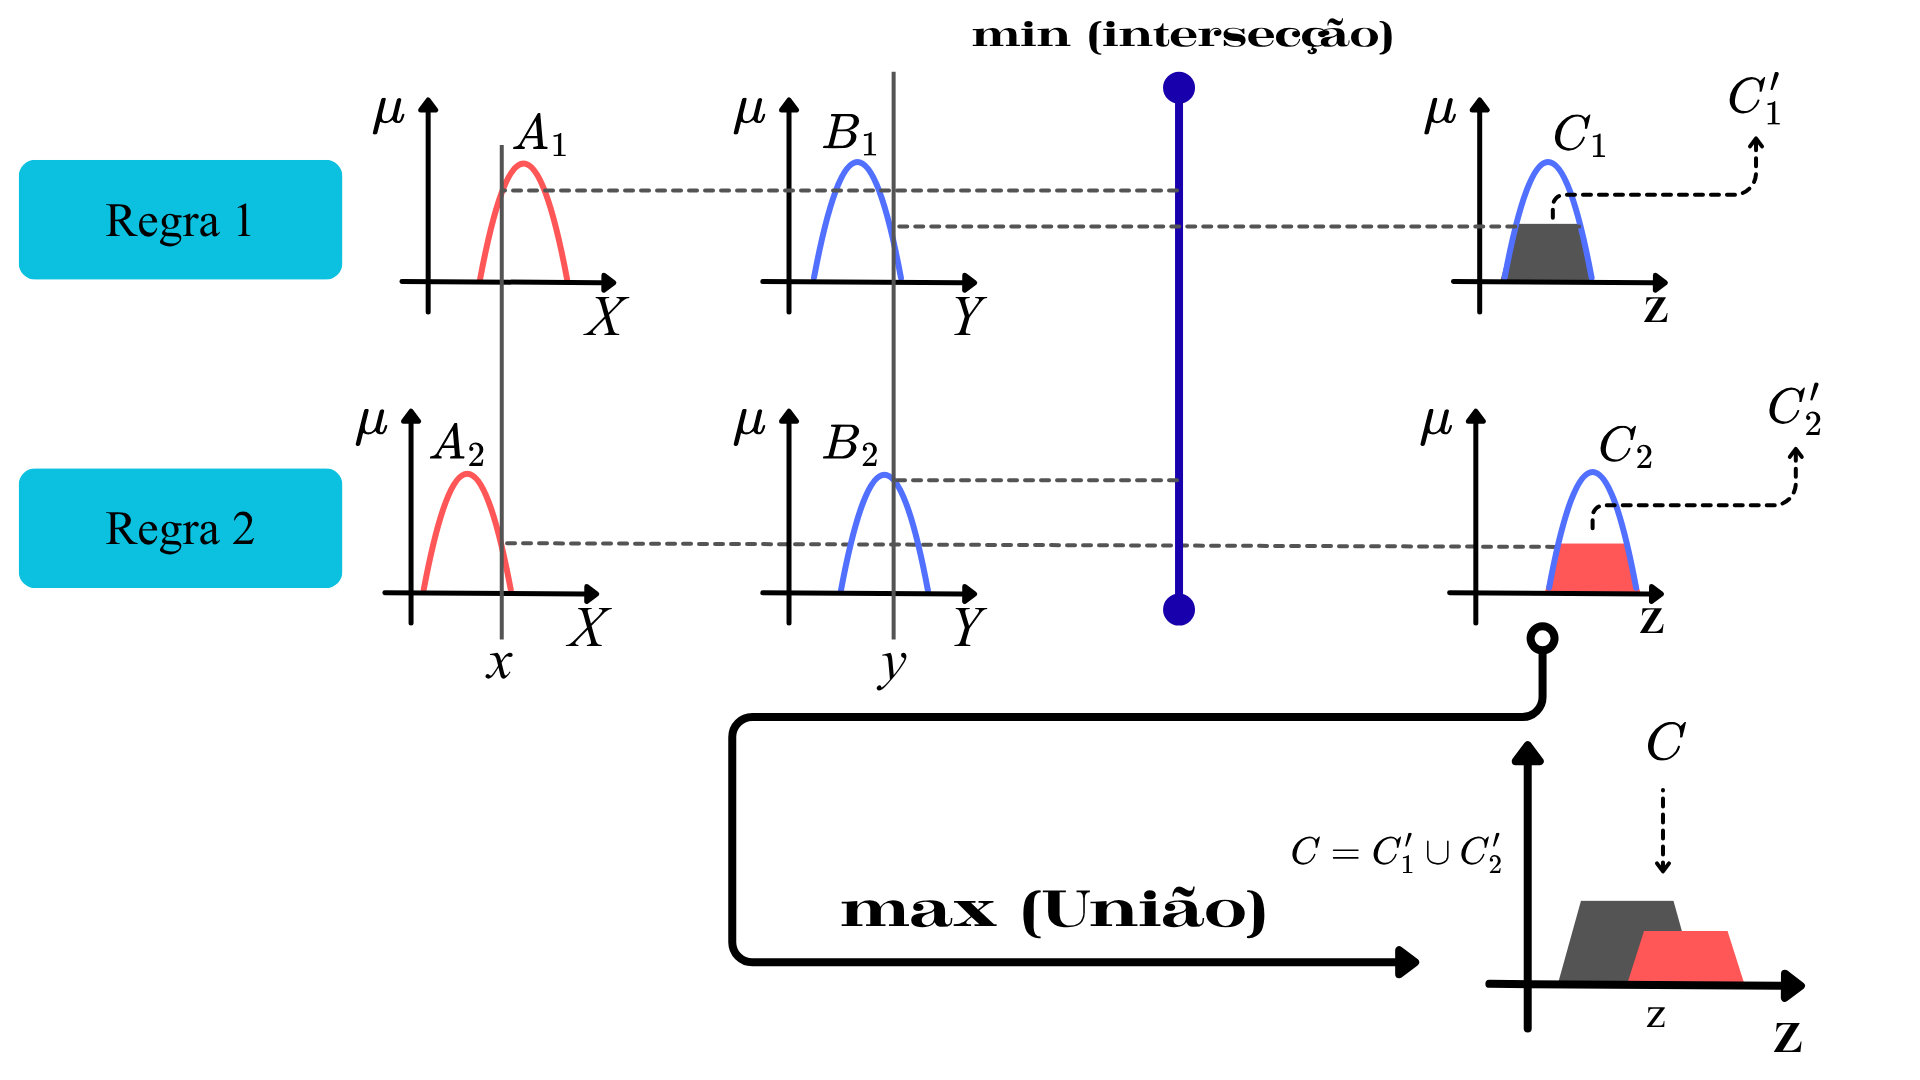
\includegraphics[width=0.7\textwidth]{figures/mamdani.png}
        %     \caption*{\footnotesize Fonte: Adaptado de \cite{fuzzy}.}
        %     \label{fig:mamdani}
        % \end{figure}
        % Com~base~no Exemplo \ref{ex:fuzzy} uma regra que poderia ser formulada:
        % $$\textbf{{\text{Regra}}  1}: \text{SE} \ (x \ \text{é} \ A) \ \text{ENTAO} \ (z \ \text{é} \ C),$$
        % em que $A$ é o conjunto fuzzy representando a categoria ``temperatura alta" e $C$ é um conjunto fuzzy representando a categoria ``baixa", da variável de saída ``temperatura do ar condicionado".
        % \begin{itemize}
        \item \textbf{Método de Takagi-Sugeno}: Neste caso, o consequente de cada regra é uma função das variáveis de entrada. Por exemplo, pode-se supor que a função que mapeia a entrada e a saída para cada regra é uma combinação linear das entradas, ou seja: 
        $$z = a_1x_1 + a_2x_2 + \cdots+ a_nx_n + b.$$ 
        Assim, as regras do método de Takagi-Sugeno podem ser formuladas da seguinte forma:
        $$
        \textbf{{\text{Regra}} r}: \text{SE}  \ x_1 \ \text{é} \ A_1 \ \text{E} \ x_2 \ \text{é} \ A_2 \cdots \ x_n \ \text{é} \ A_n \ \text{ENTAO} \ z = f_r(x_1, x_2, \ldots, x_n).
        $$
        Na Figura \ref{tks} é ilustrado um exemplo do método de Takagi-Sugeno, em que duas regras são aplicadas para inferir a saída $z$ a partir das entradas $x$ e $y$. 
        \end{itemize}
        \begin{figure}[H]
            \centering
            \caption{Exemplo de inferência fuzzy utilizando o método de Takagi-Sugeno.}
            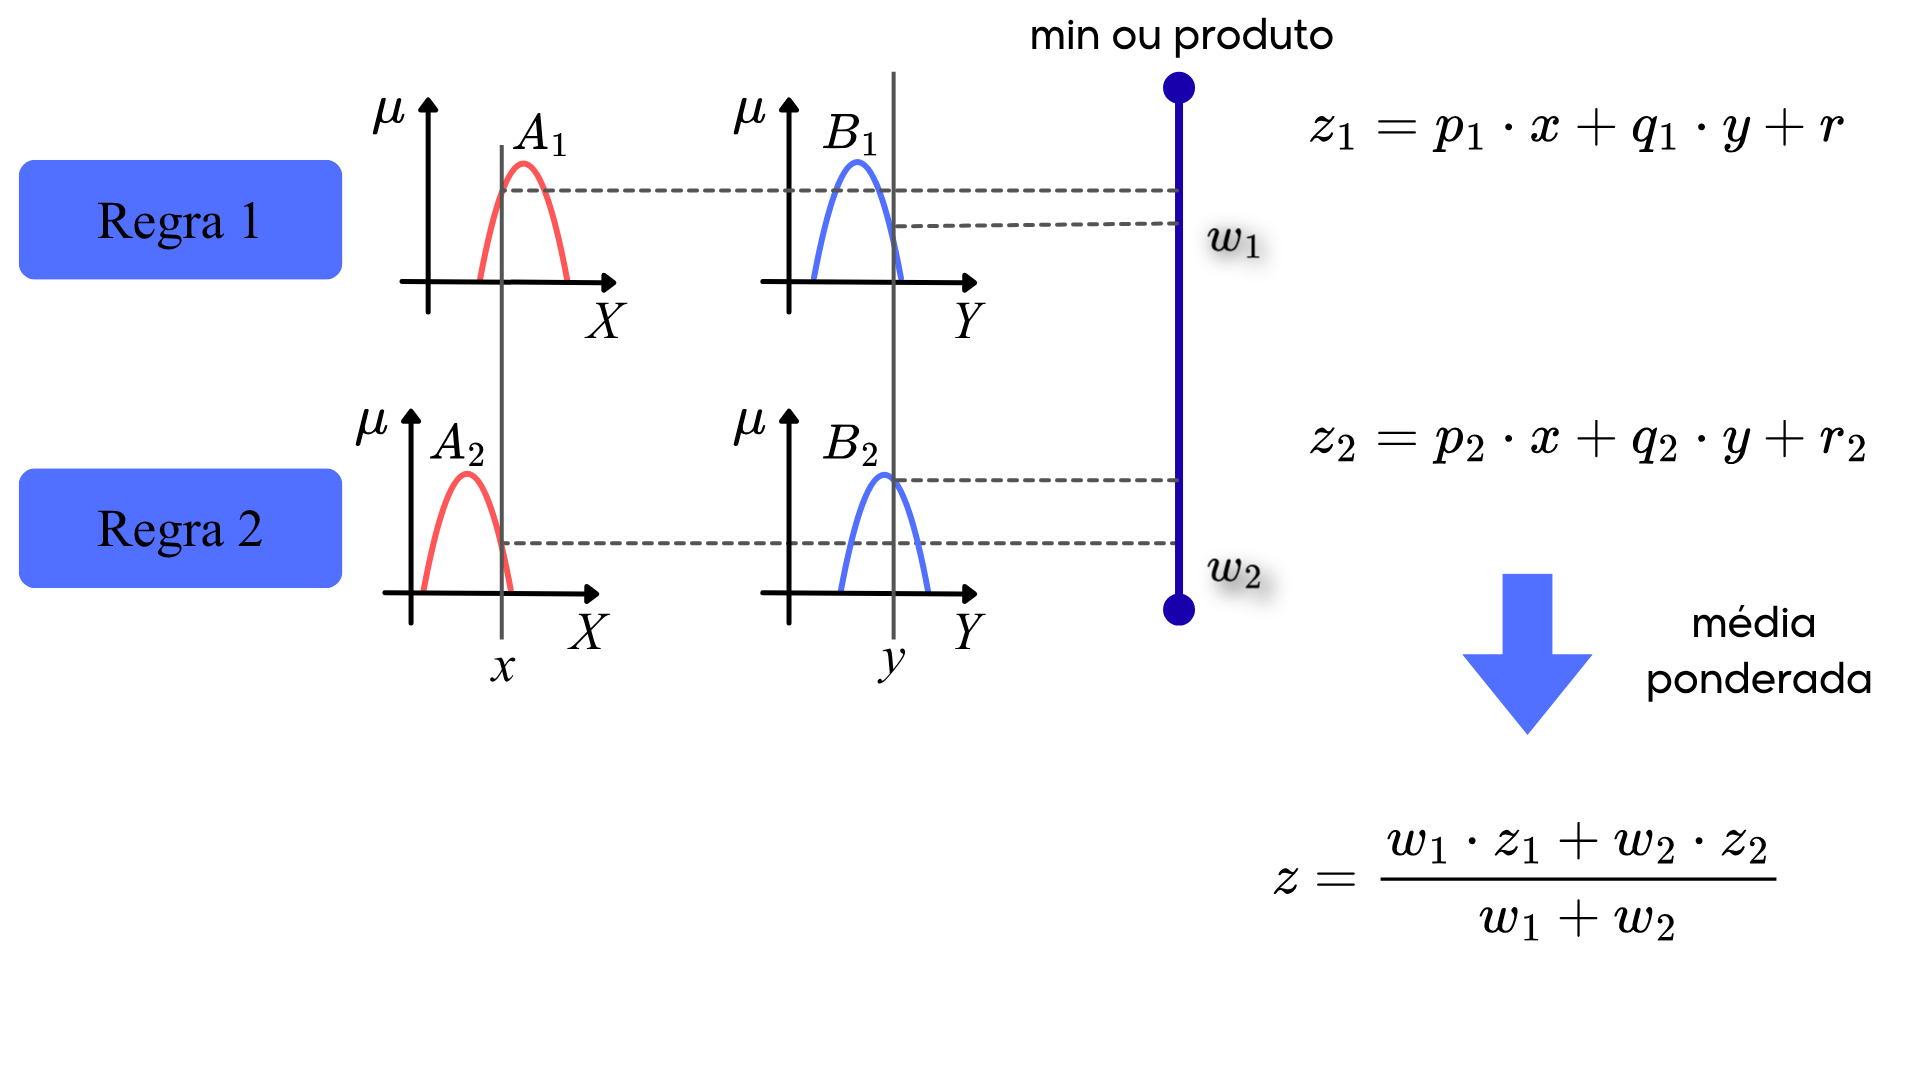
\includegraphics[width=0.7\textwidth]{figures/tks.png}
            \caption*{\footnotesize Fonte: Adaptado de \citeonline{fuzzy}.}
            \label{tks}
        \end{figure}
    
    \item A \textbf{defuzzificação} converte os conjuntos fuzzy de saída em números reais. Sistemas fuzzy, em geral, a saída é um conjunto fuzzy, assim, deve-se escolher um método de defuzzificação para obter um número real a partir do conjunto fuzzy de saída. Para o método de Takagi-Sugeno, o método de defuzzificação é dado pela média ponderada das saídas de cada regra, usando-se o grau de ativação destas regras como ponderação, ou seja:
$$z = \frac{\sum_{r=1}^R w_rf_r(x_1, x_2, \ldots, x_n)}{\sum_{r=1}^R w_r},$$
em que $R$ é o número de regras, $w_r$ é o grau de ativação da regra $r$ e $f_r(x_1, x_2, \ldots, x_n)$ é a função de saída da regra $r$. É possível observar o cálculo na Figura \ref{tks} para obter ``$z$''. 
\end{itemize}
\begin{exemplo}
Considere um sistema de controle de velocidade de um ventilador com duas variáveis de entrada: temperatura $x$ (em °C) e umidade do ar $y$ (em \%). O objetivo é determinar a velocidade $z$ do ventilador (em Rotações por Minuto - RPM) utilizando um SBRF com o método de Takagi-Sugeno.
\end{exemplo}
As variáveis linguísticas são definidas pelas seguintes funções de pertinência trapezoidais:
\begin{itemize}
    \item Temperatura ``Baixa'' ($A_1$): 
    $$
    \mu_{A_1}(x) = \begin{cases} 1, & \text{se } x \leq 20 \\ \frac{25 - x}{5}, & \text{se } 20 < x < 25 \\ 0, & \text{se } x \geq 25 \end{cases}.
    $$
    \item Temperatura ``Média'' ($A_2$):
    $$
    \mu_{A_2}(x) = \begin{cases}
        0, & \text{se} \ x < 20 \ \text{ou} \ x \geq 35 \\ \frac{x - 20}{5}, & \text{se } 20 \leq x < 25 \\ 1, & \text{se } 25 \leq x < 30 \\ \frac{35 - x}{5}, & \text{se } 30 \leq x < 35
    \end{cases}.
    $$
    \item Temperatura ``Alta'' ($A_3$): 
    $$
    \mu_{A_3}(x) = \begin{cases} 0, & \text{se } x < 30 \\ \frac{x - 30}{5}, & \text{se } 30 \leq x < 35 \\ 1, & \text{se } x \geq 35 \end{cases}.
    $$
    
    \item Umidade ``Baixa'' ($B_1$):
    $$\mu_{B_1}(y) = \begin{cases} 1, & \text{se } y <20 \\ \frac{40 - y}{20}, & \text{se } 20 \leq y < 40 \\ 0, & \text{se } y \geq 40 \end{cases}.$$
    \item Umidade ``Média'' ($B_2$): 
    $$\mu_{B_2}(y) = \begin{cases}
    0, & \text{se} \ y < 20 \ \text{ou} \ y \geq 80 \\ \frac{y - 20}{20}, & \text{se } 20 \leq y < 40 \\ 1, & \text{se } 40 \leq y < 60 \\ \frac{80 - y}{20}, & \text{se } 60 \leq y < 80
    \end{cases}.$$
    \item Umidade ``Alta'' ($B_3$):
    $$\mu_{B_3}(y) = \begin{cases} 0, & \text{se } y < 60 \\ \frac{y - 60}{20}, & \text{se } 60 \leq y < 80 \\ 1, & \text{se } y \geq 80 \end{cases}.$$

\end{itemize}

As regras fuzzy pelo método de Takagi-Sugeno são:
$$
\begin{cases}
  \textbf{Regra 1}: \text{SE } (x \text{ é } A_1 \text{ E } y \text{ é } B_1) \text{ ENTÃO } z_1 = 5x + 2y; \\
  \textbf{Regra 2}: \text{SE } (x \text{ é } A_2 \text{ E } y \text{ é } B_2) \text{ ENTÃO } z_2 = x + y; \\
  \textbf{Regra 3}: \text{SE } (x \text{ é } A_3 \text{ E } y \text{ é } B_3) \text{ ENTÃO } z_3 = 2x + 3y; \\
  \textbf{Regra 4}: \text{SE } (x \text{ é } A_1 \text{ E } y \text{ é } B_2) \text{ ENTÃO } z_4 = 3x + y; \\
  \textbf{Regra 5}: \text{SE } (x \text{ é } A_2 \text{ E } y \text{ é } B_1) \text{ ENTÃO } z_5 = 4x + 2y; \\
  \textbf{Regra 6}: \text{SE } (x \text{ é } A_3 \text{ E } y \text{ é } B_1) \text{ ENTÃO } z_6 = 2x + y; \\
  \textbf{Regra 7}: \text{SE } (x \text{ é } A_1 \text{ E } y \text{ é } B_3) \text{ ENTÃO } z_7 = 3x + 4y; \\
  \textbf{Regra 8}: \text{SE } (x \text{ é } A_2 \text{ E } y \text{ é } B_3) \text{ ENTÃO } z_8 = 4x + 3y; \\
  \textbf{Regra 9}: \text{SE } (x \text{ é } A_3 \text{ E } y \text{ é } B_2) \text{ ENTÃO } z_9 = 5x + y
\end{cases}.
$$
Para as entradas $x = 35$°C e $y = 70$\%, os graus de pertinência são:
$$\mu_{A_1}(35) = 0, \quad \mu_{A_2}(35) = 0, \quad \mu_{A_3}(35) = 1.$$
$$\mu_{B_1}(70) = 0, \quad \mu_{B_2}(70) = 0{,}5, \quad \mu_{B_3}(70) = 0{,}5.$$

Os graus de ativação de cada regra, utilizando o operador do mínimo, são:
$$
\begin{cases}
    w_1 = \min(\mu_{A_1}(35),\ \mu_{B_1}(70)) = \min(0;\ 0) = 0;\\
    w_2 = \min(\mu_{A_2}(35),\ \mu_{B_2}(70)) = \min(0;\ 0{,}5) = 0;\\
    w_3 = \min(\mu_{A_3}(35),\ \mu_{B_3}(70)) = \min(1;\ 0{,}5) = 0{,}5;\\
    w_4 = \min(\mu_{A_1}(35),\ \mu_{B_2}(70)) = \min(0;\ 0{,}5) = 0;\\
    w_5 = \min(\mu_{A_2}(35),\ \mu_{B_1}(70)) = \min(0;\ 0) = 0;\\
    w_6 = \min(\mu_{A_3}(35),\ \mu_{B_1}(70)) = \min(1;\ 0) = 0;\\
    w_7 = \min(\mu_{A_1}(35),\ \mu_{B_3}(70)) = \min(0;\ 0{,}5) = 0;\\
    w_8 = \min(\mu_{A_2}(35),\ \mu_{B_3}(70)) = \min(0;\ 0{,}5) = 0;\\
    w_9 = \min(\mu_{A_3}(35),\ \mu_{B_2}(70)) = \min(1;\ 0{,}5) = 0{,}5.\\
\end{cases}
$$
As saídas de cada regra são:
$$
\begin{cases}
z_1 = 5 \cdot 35 + 2 \cdot 70 = 315; \\
z_2 = 35 + 70 = 105; \\
z_3 = 2 \cdot 35 + 3 \cdot 70 = 280; \\
z_4 = 3 \cdot 35 + 70 = 175; \\
z_5 = 4 \cdot 35 + 2 \cdot 70 = 280; \\
z_6 = 2 \cdot 35 + 70 = 140; \\
z_7 = 3 \cdot 35 + 4 \cdot 70 = 385; \\
z_8 = 4 \cdot 35 + 3 \cdot 70 = 350; \\
z_9 = 5 \cdot 35 + 70 = 245.
\end{cases}
$$
A saída final é obtida pela média ponderada:
$$z = \frac{w_1 \cdot z_1 + w_2 \cdot z_2 + w_3 \cdot z_3 + w_4 \cdot z_4 + w_5 \cdot z_5 + w_6 \cdot z_6 + w_7 \cdot z_7 + w_8 \cdot z_8 + w_9 \cdot z_9}{w_1 + w_2 + w_3 + w_4 + w_5 + w_6 + w_7 + w_8 + w_9} = 
$$
$$
\frac{0 \cdot 315 + 0 \cdot 105 +  0{,}5 \cdot 280 + 0 \cdot 175 + 0 \cdot 280 + 0 \cdot 140 + 0 \cdot 385 + 0 \cdot 350 + 0{,}5 \cdot 245}{0 + 0 + 0{,}5 + 0 + 0 + 0 + 0 + 0 + 0{,}5} =
$$ 

$$= \frac{140 + 122{,}5}{1} =  262{,}5 \text{ RPM}.
$$

Portanto, para uma temperatura de $35$°C e umidade do ar de $70$\%, o sistema baseado em regrás fuzzy com o método de Takagi-Sugeno determina que a velocidade do ventilador deve ser de $262{,}5$ RPM, uma boa velocidade para refrescar o ambiente.


\section{ANFIS}
\label{anfis}
O Sistema Adaptativo de Inferência Neuro-Fuzzy, do inglês \textit{Adaptative Neuro-Fuzzy Inference System - ANFIS}, é uma técnica híbrida em inteligência artificial, que combina a capacidade de aprendizado das redes neurais artificiais com a representação de conhecimento e raciocínio aproximado dos sistemas baseados em regras fuzzy \cite{fuzzy}. Essa abordagem permite determinar um SBRF a partir de conhecimentos obtidos por meio de um processo de treinamento, utilizando um conjunto de dados de entrada e saída, sendo o principal método de inferência utilizado o método de Takagi-Sugeno \cite{Jang1993}. 

O ANFIS é composto por cinco camadas, cada uma com uma função específica. Para exemplificar cada camada, considere o sistema com duas entradas, $x_1$ e $x_2$, e uma saída $y$, com quatro regras fuzzy do tipo Takagi-Sugeno, ou seja:
\begin{center}
\textbf{Regra 1}: SE $x_1$ é $A^{(1)}_1$ E $x_2$ é $A^{(2)}_1$ ENTÃO $y = f_{1,1}(x_1, x_2) = k_{10} + k_{11}x_1 + k_{12}x_2$; \\
\textbf{Regra 2}: SE $x_1$ é $A^{(1)}_1$ E $x_2$ é $A^{(2)}_2$ ENTÃO $y = f_{1,2}(x_1, x_2) = k_{20} + k_{21}x_1 + k_{22}x_2$; \\
\textbf{Regra 3}: SE $x_1$ é $A^{(1)}_2$ E $x_2$ é $A^{(2)}_1$ ENTÃO $y = f_{2,1}(x_1, x_2) = k_{30} + k_{31}x_1 + k_{32}x_2$; \\
\textbf{Regra 4}: SE $x_1$ é $A^{(1)}_2$ E $x_2$ é $A^{(2)}_2$ ENTÃO $y = f_{2,2}(x_1, x_2) = k_{40} + k_{41}x_1 + k_{42}x_2$.
\end{center}
em que $A^{(1)}_1, A^{(1)}_2$ são os conjuntos fuzzy do universo $X_1$, associados à variável de entrada $x_1$ e $A^{(2)}_1, A^{(2)}_2$ são os conjuntos fuzzy do universo $X_2$, associados à variável de entrada $x_2$; e $k_{i0}, k_{i1}, k_{i2}$ são os parâmetros de cada regra, para $i = 1, 2, 3, 4$. Para este exemplo, considera-se que as funções de pertinência dos conjuntos fuzzy $A^{(1)}_j$ e $A^{(2)}_j$ são gaussianas, definidas pela Equação (\ref{eq:gaussiana}).

Na primeira camada os valores de entrada são transformados em graus de pertinência dos conjuntos fuzzy, ou seja:
$$
\begin{cases}
y^{(1)}_i = \mu_{A^{(1)}_i}(x_1); \\    
\ y^{(1)}_{i+2} = \mu_{A^{(2)}_i}(x_2)
\end{cases},
$$
para $i = 1, 2$. 

Na segunda camada, as regras fuzzy são criadas com base no operador lógico ``E'' definido por uma t-norma, ou seja:
$$\begin{cases}
y^{(2)}_{1,1} = w_{1,1} = \mu_{A^{(1)}_1}(x_1) \cdot \mu_{A^{(2)}_1}(x_2); \\
y^{(2)}_{1,2} = w_{1,2} = \mu_{A^{(1)}_1}(x_1) \cdot \mu_{A^{(2)}_2}(x_2); \\
y^{(2)}_{2,1} = w_{2,1} = \mu_{A^{(1)}_2}(x_1) \cdot \mu_{A^{(2)}_1}(x_2); \\
y^{(2)}_{2,2} = w_{2,2} = \mu_{A^{(1)}_2}(x_1) \cdot \mu_{A^{(2)}_2}(x_2)
\end{cases};$$
em que $w_{h,j}$ é o peso de ativação da regra associada à combinação $(A^{(1)}_h, A^{(2)}_j)$, para $h, j = 1, 2$. Na terceira camada os pesos de cada regra são normalizados, ou seja:
$$
y^{(3)}_{h,j} = \bar{w}_{h,j} = \frac{w_{h,j}}{w_{1,1} + w_{1,2} + w_{2,1} + w_{2,2}};
$$
para $h, j = 1, 2$. Na quarta camada a parte ``ENTÃO'' das regras fuzzy são criadas, ou seja:
$$
y^{(4)}_{h,j} = \bar{w}_{h,j} f_{h,j} = \bar{w}_{h,j} (k_{h0} + k_{h1}x_1 + k_{h2}x_2)
$$
Para a última camada, a saída é obtida pela média ponderada:
$$y = \frac{\sum_{h=1}^{2} \sum_{j=1}^{2} \bar{w}_{h,j} f_{h,j}}{\sum_{h=1}^{2} \sum_{j=1}^{2} \bar{w}_{h,j}}.$$

Na Figura \ref{img:anfis} é ilustrada a arquitetura do ANFIS para o exemplo apresentado. As setas na Figura \ref{img:anfis} representam as conexões entre as camadas do ANFIS. Observa-se que para dois antecedentes, $x_1$ e $x_2$, e dois conjuntos fuzzy para cada antecedente, $A^{(1)}_1, A^{(1)}_2$ e $A^{(2)}_1, A^{(2)}_2$, são criadas quatro regras fuzzy, ou seja, $n^k = 2^2 = 4$ regras fuzzy. Para um número geral de $k$ antecedentes e $n$ conjuntos fuzzy para cada antecedente, o número de regras fuzzy criadas é dado por $n^k$.
\begin{figure}[H]
    \centering
    \caption{Arquitetura do ANFIS}
    
\includegraphics[width=0.8\textwidth]{cap2/anfis.png}
    \caption*{\footnotesize Fonte: Adaptado de \citeonline{fuzzy}.}
    \label{img:anfis}
\end{figure}

Neste capítulo foram apresentados os principais conceitos relacionados à teoria fuzzy, iniciando com a definição de conjuntos fuzzy e terminando com a definição da ANFIS. No próximo capítulo, é introduzida a principal rede neural utilizada neste trabalho.


% $$
% \begin{cases}
% y_i^{(1)} = \mu_{A^{(1)}_i}(x_1) \text{ para } i = 1, 2, \ldots, n; \\
% y_{i+n}^{(1)} = \mu_{A^{(2)}_i}(x_2) \text{ para } i = 1, 2, \ldots, n; \\
% \vdots \\
% y_{i+n(k-1)}^{(1)} = \mu_{A^{(k)}_i}(x_k) \text{ para } i = 1, 2, \ldots, n,
% \end{cases}
% $$
% em que $x_1$ é a entrada e $\mu_{A^{(k)}_i}$ são as funções de pertinência dos conjuntos fuzzy $A^{(k)}_i$ associados à variável de entrada $x_k$ e $k \in \mathbb{N}$. As funções de pertinência utilizadas são as gaussianas, definidas pela Equação (\ref{eq:gaussiana}).

% Na \textbf{segunda camada} a parte ``SE'' das regras fuzzy são criadas com base no operador lógico ``E'' definido por uma t-norma, ou seja:
% $$
% \begin{cases}
% y_1^{(2)} = w_{1,1,\ldots,1} = \prod_{\ell=1}^{k} \mu_{A^{(\ell)}_1}(x_\ell); \\
% y_2^{(2)} = w_{1,1,\ldots,2} = \mu_{A^{(1)}_1}(x_1)\mu_{A^{(2)}_1}(x_2) \cdots \mu_{A^{(k)}_2}(x_k); \\
% \vdots \\
% y_{n^k}^{(2)} = w_{n,n,\ldots,n} = \prod_{\ell=1}^{k} \mu_{A^{(\ell)}_n}(x_\ell),
% \end{cases}
% $$
% ou, de forma geral,
% $$
% w_{i_1, i_2, \ldots, i_k} = \prod_{\ell=1}^{k} \mu_{A^{(\ell)}_{i_\ell}}(x_\ell), \qquad i_\ell \in \{1, 2, \ldots, n\}.
% $$
% em que $w_{i_1, i_2, \ldots, i_k}$ é o peso de ativação da regra associada à combinação $(A^{(1)}_{i_1}, A^{(2)}_{i_2}, \ldots, A^{(k)}_{i_k})$, totalizando $n^k$ regras fuzzy.
% Na \textbf{terceira camada} os pesos de cada regra são normalizados, ou seja:
% $$\begin{cases}
% y_1^{(3)} = \bar{w}_{1,1,\ldots,1} = \frac{w_{1,1,\ldots,1}}{\sum_{j_1=1}^{n} \sum_{j_2=1}^{n} \cdots \sum_{j_k=1}^{n} w_{j_1, j_2, \ldots, j_k}}; \\
% y_2^{(3)} = \bar{w}_{1,1,\ldots,2} = \frac{w_{1,1,\ldots,2}}{\sum_{j_1=1}^{n} \sum_{j_2=1}^{n} \cdots \sum_{j_k=1}^{n} w_{j_1, j_2, \ldots, j_k}}; \\
% \vdots \\
% y_{n^k}^{(3)} = \bar{w}_{n,n,\ldots,n} = \frac{w_{n,n,\ldots,n}}{\sum_{j_1=1}^{n} \sum_{j_2=1}^{n} \cdots \sum_{j_k=1}^{n} w_{j_1, j_2, \ldots, j_k}}.
% \end{cases}$$

% Na \textbf{quarta camada} a parte ``ENTÃO'' das regras fuzzy são criadas, utilizando o método de Takagi-Sugeno, ou seja:
% $$\begin{cases}
% y_1^{(4)} = \bar{w}_{1,1,\ldots,1} f_{1,1,\ldots,1}; \\
% y_2^{(4)} = \bar{w}_{1,1,\ldots,2} f_{1,1,\ldots,2}; \\
% \vdots \\
% y_{n^k}^{(4)} = \bar{w}_{n,n,\ldots,n} f_{n,n,\ldots,n},
% \end{cases}$$
% em que
% $$
% f_{i_1, i_2, \ldots, i_k}(x_1, x_2, \ldots, x_k) = a_{i_1, i_2, \ldots, i_k, 1}x_1 + a_{i_1, i_2, \ldots, i_k, 2}x_2 + \cdots + a_{i_1, i_2, \ldots, i_k, k}x_k + b_{i_1, i_2, \ldots, i_k}.
% $$
% Na \textbf{quinta camada} a saída do sistema é calculada pela média ponderada das saídas de cada regra, utilizando os pesos normalizados como ponderação, ou seja:
% $$
% y^{(5)} = \sum_{i_1=1}^{n} \sum_{i_2=1}^{n} \cdots \sum_{i_k=1}^{n} \bar{w}_{i_1, i_2, \ldots, i_k} f_{i_1, i_2, \ldots, i_k}.
% $$

